\documentclass{beamer}
\usepackage{hyperref}
\usepackage[T1]{fontenc}

% other packages
\usepackage{latexsym, amsmath, xcolor, multicol, multirow, booktabs}
\usepackage{graphicx, pstricks, listings, stackengine}
\usepackage{soul}

% packages and settings for bibtex
\usepackage[backend=bibtex, sorting=none]{biblatex}
\addbibresource{ref.bib}
\setbeamerfont{footnote}{size=\tiny}   % footnote for bibtex
\setbeamertemplate{bibliography item}[text]   % reference list for bibtex
\defbibheading{reference}{\section*{References}}   % heading for bibtex

\author[Calvin Massonnet]{Calvin Massonnet\\{\small calvin.massonnet@etu.univ-grenoble-alpes.fr}}
\title{Multi-agent simulation of trust in vaccination}
\subtitle{Project presentation}
\institute{Internship funded by CNRS MODCOV19\\
Supervised by Carole ADAM (LIG) and Didier GEAORGES (GIPSA-lab)\\
With the help of Pierrick TRANOUEZ (Litis, Université Rouen Normandie)}  % Université Grenoble Alpes
\date{Masters defence - 1\textsuperscript{st} of September 2022}  % \today
\usepackage{ucas}

% defs
\def\cmd#1{\texttt{\color{red}\footnotesize $\backslash$#1}}
\def\env#1{\texttt{\color{blue}\footnotesize #1}}
\definecolor{deepblue}{rgb}{0,0,0.5}
\definecolor{deepred}{rgb}{0.6,0,0}
\definecolor{deepgreen}{rgb}{0,0.5,0}
\definecolor{halfgray}{gray}{0.55}

\newcommand{\vcenteredhbox}[1]{\begingroup
\setbox0=\hbox{#1}\parbox{\wd0}{\box0}\endgroup}

\lstset{
    basicstyle=\ttfamily\small,
    keywordstyle=\bfseries\color{deepblue},
    emphstyle=\ttfamily\color{deepred},    % Custom highlighting style
    stringstyle=\color{deepgreen},
    numbers=left,
    numberstyle=\small\color{halfgray},
    rulesepcolor=\color{red!20!green!20!blue!20},
    frame=shadowbox,
}


\begin{document}

\begin{frame}
    \titlepage
    \begin{figure}[htpb]
        \begin{center}
            \includegraphics[width=0.1\linewidth]{fig/logos/Logo_Université_Grenoble_Alpes_2020.svg.png}\quad\quad
            
\includegraphics[width=0.1\linewidth]{fig/logos/logo_Grenoble_INP.png}\quad\quad
            
\includegraphics[width=0.1\linewidth]{fig/logos/logo_cnrs.png}\quad\quad
            
\includegraphics[width=0.1\linewidth]{fig/logos/Logo_LIG.png}\quad\quad
            
\includegraphics[width=0.1\linewidth]{fig/logos/Logo_GIPSA-lab_Grenoble.jpg}
        \end{center}
    \end{figure}
\end{frame}


\begin{frame}
    \tableofcontents[sectionstyle=show, subsectionstyle=show/shaded/hide, subsubsectionstyle=show/shaded/hide]
\end{frame}


\section{Introduction}

\begin{frame}{Vaccine hesitancy}
    Influencing factors:
    \begin{itemize}
        \item Complacency
        \item Fear of needles
        \item Lack of proper scientific background
        \item Distrust of public authorities
        \item Deaths from vaccine-preventable diseases
    \end{itemize}
    \pause
    \vspace{1.5\baselineskip}
    COVID-19 vaccine additional influencing factors:
    \begin{itemize}
        \item Early vaccine roll-out
        \item "New" vaccine technology
    \end{itemize}
\end{frame}

% Ces facteurs d'influences peuvent être parés en informant la population...
% Cette ambiguïtée dans l'information apporte, chez le public, une mésinterprétation...
\begin{frame}{Misleading information and misinterpretation}
    \begin{figure}[htpb]
        \begin{center}
            \vcenteredhbox{
\includegraphics[width=0.4\linewidth]{fig/bfmtv_tweet.png}}
            \footnote{{\tiny \url{https://twitter.com/BFMTV/status/1471539246985060360}}}
            \vcenteredhbox{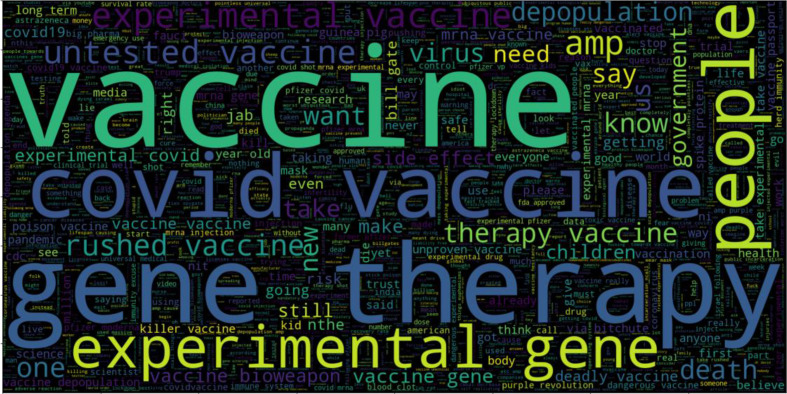
\includegraphics[width=0.7\linewidth]{fig/antivax_twitter_data.jpg}}
            \footnote{{\tiny \url{https://www.ncbi.nlm.nih.gov/pmc/articles/PMC8648668/}}}
            \\Word cloud visualization for vaccine misinformation tweets
        \end{center}
    \end{figure}
\end{frame}

% Diminution de la confiance de la population causée par ...
\begin{frame}{Problem}
    Misleading information and misinterpretation of information
    \begin{itemize}
        \item Decrease in the population's trust
    \end{itemize}
    \vspace{1.5\baselineskip}
    Effects of the decrease
    \begin{itemize}
        \item Lower trust in vaccines and institutions
        \item Lower vaccination rates
    \end{itemize}
\end{frame}

\begin{frame}{Goal}
    Educational simulation
    \begin{itemize}
        \item Agent-based simulations on vaccine effectiveness
        \item Public trust in vaccines
        \item Computer Science, Psychology, and Epidemiology
    \end{itemize}
    \vspace{2\baselineskip}
    In the continuity of \href{https://covprehension.org/}{\ul{CoVprehension}}
    \vspace{\baselineskip}
    \\GRETSI'22 presentation by Pierrick TRANOUEZ
\end{frame}



\section{State-of-the-art}

\begin{frame}{Epidemic simulations - Mathematical models}
    \begin{figure}[htpb]
        \begin{center}
            \vcenteredhbox{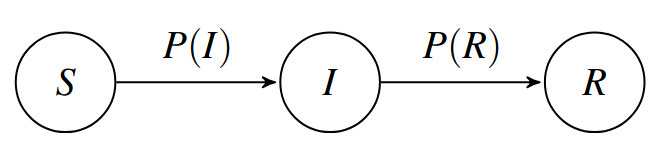
\includegraphics[width=0.4\linewidth]{fig/SIR_diagram.png}}
            \vcenteredhbox{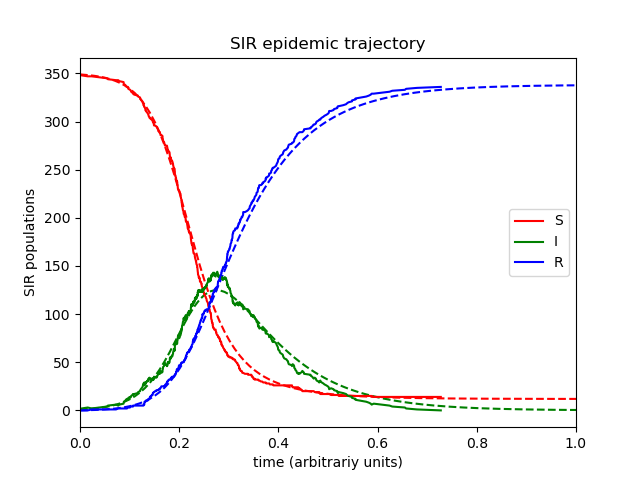
\includegraphics[width=0.5\linewidth]{fig/SIR_graph.png}}
            \footnote{{\tiny \url{https://en.wikipedia.org/wiki/Compartmental_models_in_epidemiology}}}
        \end{center}
    \end{figure}
\end{frame}

\begin{frame}{Epidemic simulations - Agent-based models (ABM)}
    \begin{figure}[htpb]
        \begin{center}
            \vcenteredhbox{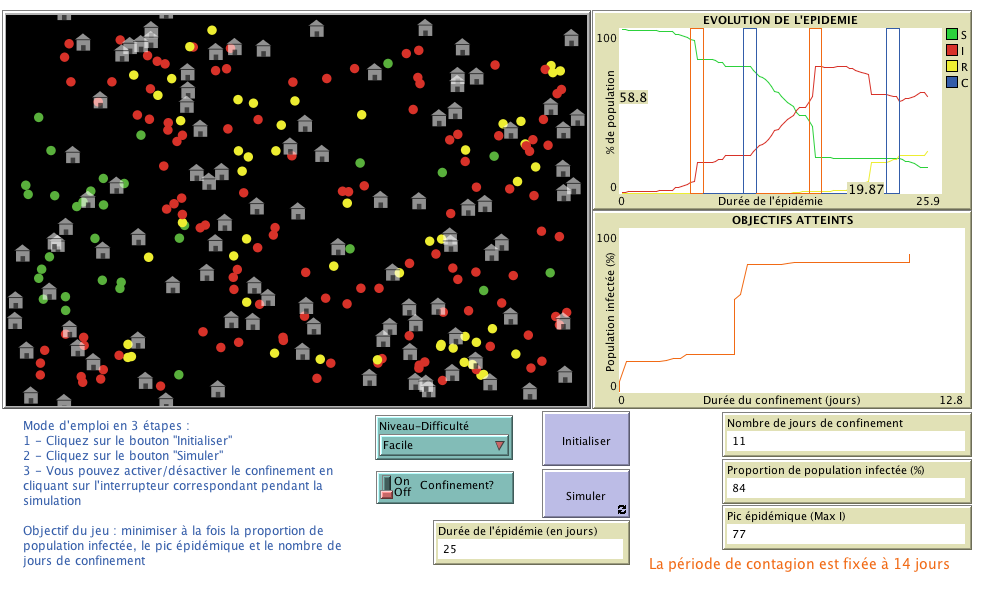
\includegraphics[width=0.8\linewidth]{fig/abm_covprehension_q6.png}}
            \footnote{{\tiny \url{https://covprehension.org/2020/03/30/q6.html}}}
        \end{center}
    \end{figure}
\end{frame}

\begin{frame}{Epidemic simulations}
    \begin{columns}
        \begin{column}{0.5\textwidth}
            Mathematical models
            \begin{itemize}
                \item Homogeneous
                \item Macro-level model
                \item Macro-level analysis
            \end{itemize}
        \end{column}
        \begin{column}{0.5\textwidth}
            Agent-based models
            \begin{itemize}
                \item Heterogeneous
                \item Micro-level model
                \item Micro \& Macro-level analysis
            \end{itemize}
        \end{column}
    \end{columns}
\end{frame}



\section{Conceptual model}

\begin{frame}{Agent attributes}
    \begin{itemize}
        \item Epidemiological state
        \item Vaccine status (boolean)
        \item Trust level (float: 0.0 - 1.0)
        \item Misinterpretation status (boolean)
    \end{itemize}
\end{frame}

\begin{frame}{Epidemiological model}
    \begin{figure}
        \begin{center}
            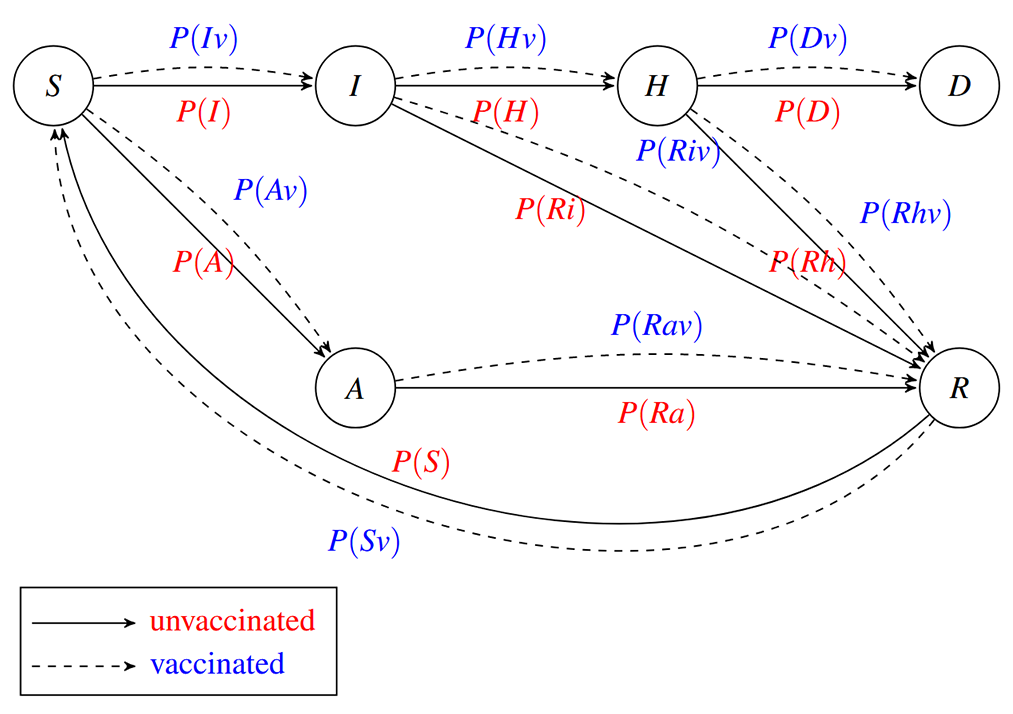
\includegraphics[width=0.8\linewidth]{fig/SIAHRD.png}
        \end{center}
    \end{figure}
    S: Susceptible; I: Symptomatic; A: Asymptomatic; H: Hospitalised; R: Recovered; D: Deceased
\end{frame}

\begin{frame}{Agent behaviour}
    \begin{itemize}
        \item Move randomly
        \item Hospitalised are put apart
        \item Susceptible, Asymptomatic \& Recovered visit hospitalised
        \item Uninfected get vaccinated based on their trust level
    \end{itemize}
    \vspace{1.5\baselineskip}
    Three influence over trust:
    \begin{itemize}
        \item Interpersonal
        \item Observational
        \item Institutional
    \end{itemize}
\end{frame}

\begin{frame}{Interpersonal influence}
    \begin{figure}[htpb]
        \begin{center}
            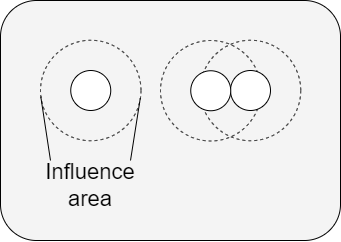
\includegraphics[width=0.4\linewidth]{fig/interpersonal.drawio.png}
        \end{center}
    \end{figure}
    \begin{table}[]
        \centering
        \begin{tabular}{|c|c|l|l}
        \cline{1-3}
        \multicolumn{1}{|l|}{\textbf{\begin{tabular}[c]{@{}l@{}}Agent A's\\ trust level\end{tabular}}} &
        \multicolumn{1}{l|}{\textbf{\begin{tabular}[c]{@{}l@{}}Agent B's\\ trust level\end{tabular}}} &
        \textbf{Resulting influence} &
        \\ \cline{1-3}
            0.9 & 0.5 & High influence of A over B     &  \\ \cline{1-3}
            0.9 & 0.8 & Mutual confirmation            &  \\ \cline{1-3}
            0.9 & 0.3 & A less influenced than B       &  \\ \cline{1-3}
            0.9 & 0.1 & Influence almost cancelled out &  \\ \cline{1-3}
        \end{tabular}
    \end{table}
\end{frame}

\begin{frame}{Observational influence}
    \begin{figure}[htpb]
        \begin{center}
            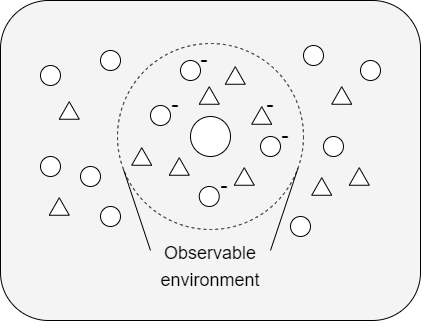
\includegraphics[width=0.5\linewidth]{fig/observational.drawio.png}
        \end{center}
    \end{figure}
    \begin{table}[]
        \centering
        \begin{tabular}{lll}
        \cline{1-2}
        \multicolumn{1}{|l|}{\textbf{Agent's observation}} & \multicolumn{1}{l|}{\textbf{Resulting influence}} &  \\ \cline{1-2}
        \multicolumn{1}{|l|}{Vaccinated and not infected} & \multicolumn{1}{l|}{Small increase in observer's trust} &  \\ \cline{1-2}
        \multicolumn{1}{|l|}{Vaccinated and infected} & \multicolumn{1}{l|}{Decrease in observer's trust} &  \\ \cline{1-2}
        \end{tabular}
    \end{table}
    \textit{Negative information have more impact than positive information}
\end{frame}

\begin{frame}{Institutional influence and misinterpretation}
    \begin{figure}[htpb]
        \begin{center}
            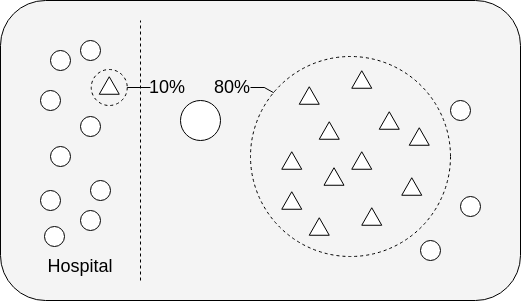
\includegraphics[width=0.6\linewidth]{fig/institutional.drawio.png}
        \end{center}
    \end{figure}
\end{frame}



\section{Implementation}

\begin{frame}{Details}
    \begin{itemize}
        \item NetLogo
        \item $\sim$800 lines
        \item Based on CoVprehension's Q17
        \item Available on \href{https://github.com/CalvinMT/TrustVaccSim}{\ul{GitHub}}
        \item Runnable on \href{https://www.netlogoweb.org/launch\#https://raw.githubusercontent.com/CalvinMT/TrustVaccSim/main/src/trustvaccsim.nlogo}{\ul{NetLogo Web}}
    \end{itemize}
\end{frame}

\begin{frame}{Simulation environment}
    \begin{figure}
        \begin{center}
            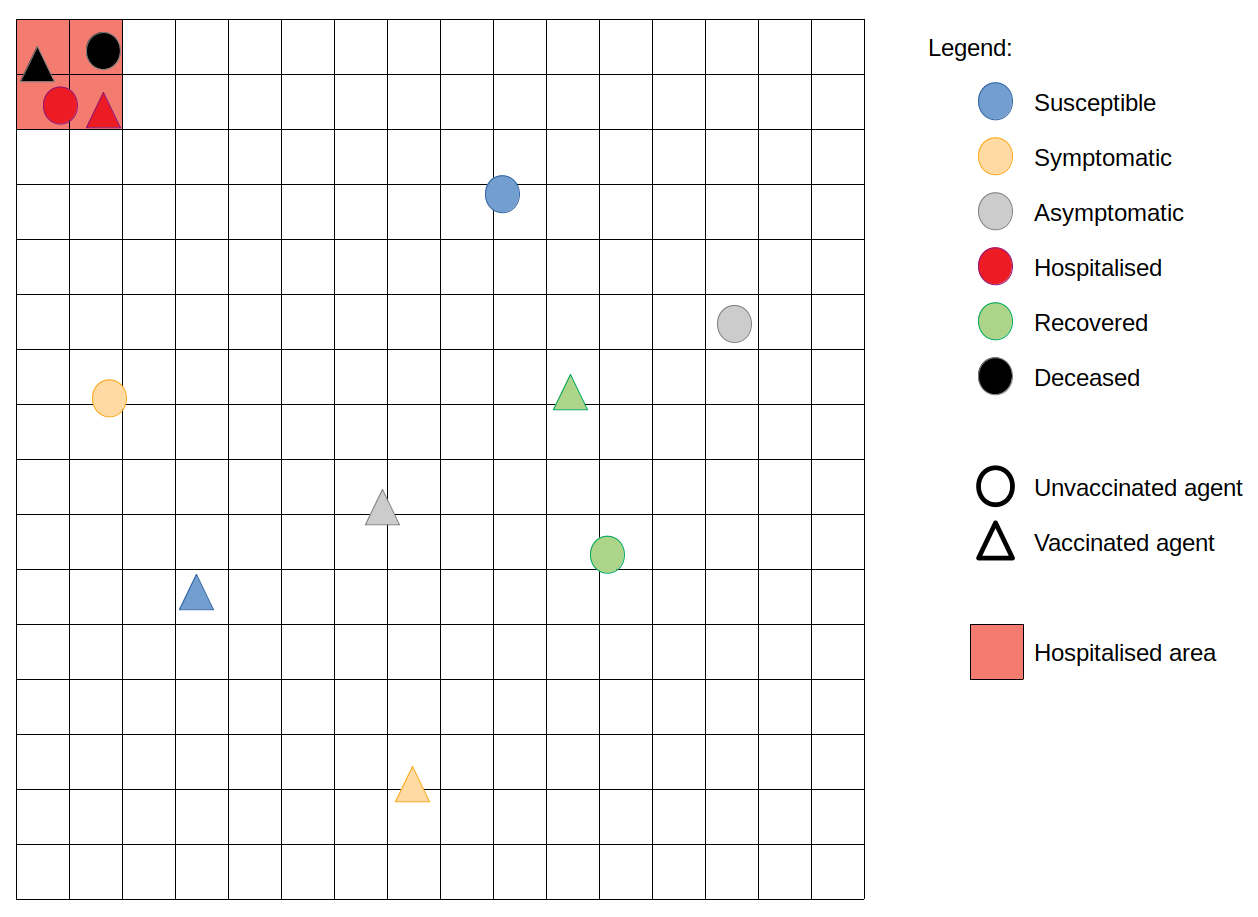
\includegraphics[width=0.8\linewidth]{fig/simulation_figure.png}
        \end{center}
    \end{figure}
\end{frame}

\begin{frame}{Environment details}
    \begin{itemize}
        \item 2000 agents
        \item Agents initialised unvaccinated
        \item Agents initialised as Susceptible
        \item One agent initialised as Symptomatic
        \item Trust initialised randomly following custom law similar to a skew normal distribution
    \end{itemize}
    \begin{figure}
        \begin{center}
            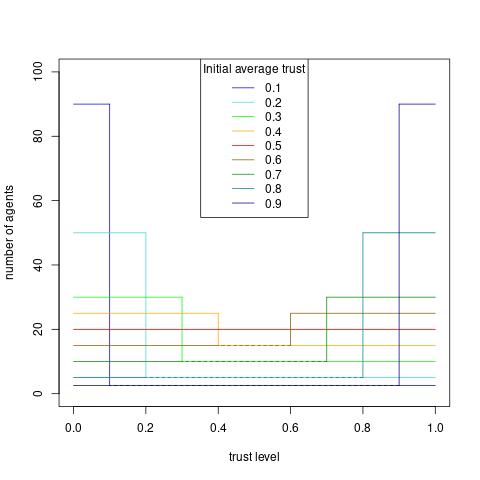
\includegraphics[width=0.3\linewidth]{fig/initial_average_trust.png}
        \end{center}
        \caption{Output of the algorithm used in the initialisation of the population's average trust.}
    \end{figure}
\end{frame}

\begin{frame}{Inputs \& Outputs}
    Input:
    \begin{itemize}
        \item Population average initial trust (0.1 - 0.9)
    \end{itemize}
    Outputs:
    \begin{itemize}
        \item Trust level per misinterpretation status
        \item Deceased per vaccination \& per misinterpretation status
    \end{itemize}
    \begin{figure}
        \begin{center}
            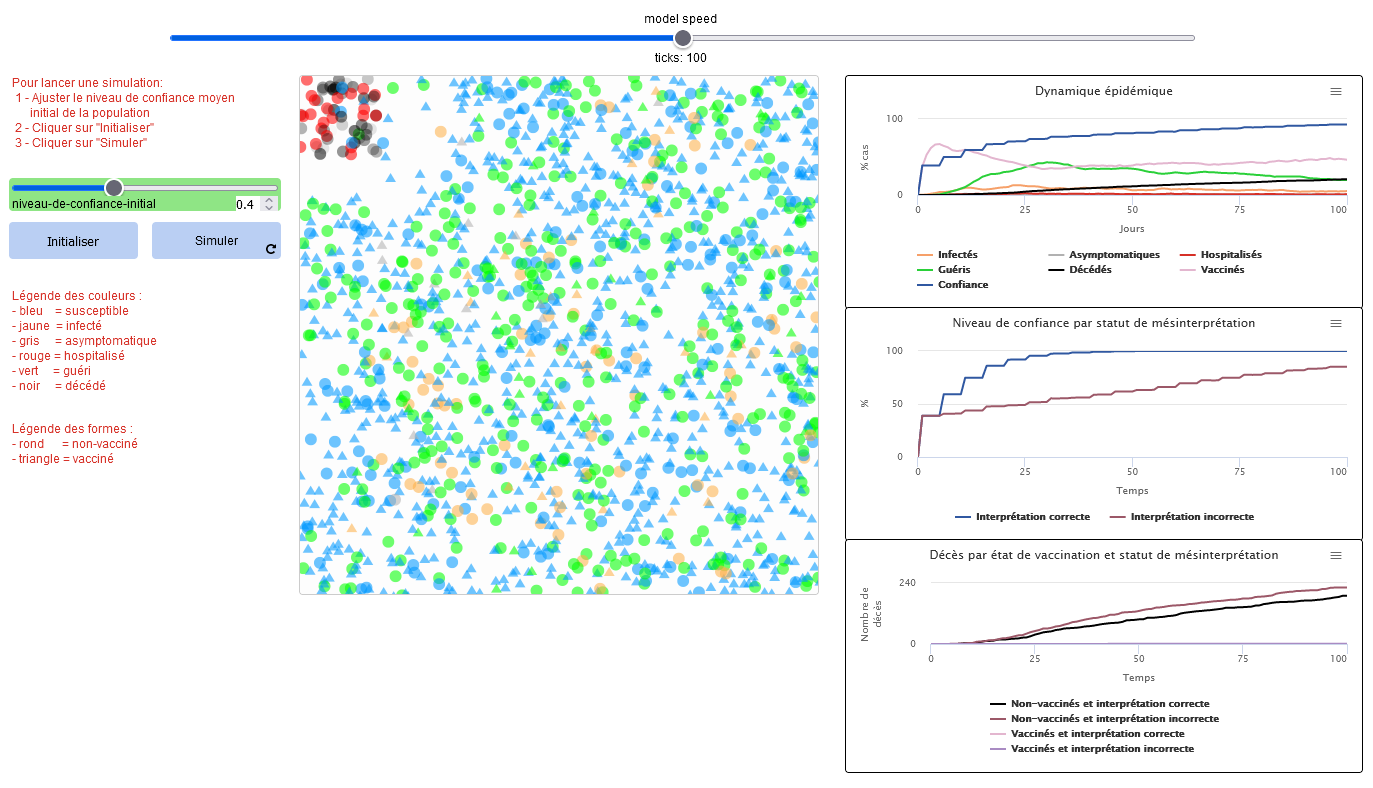
\includegraphics[width=0.7\linewidth]{fig/simulation_user_layout.png}
        \end{center}
    \end{figure}
\end{frame}



\section{Key observations}

\begin{frame}{Trust and misinterpretation}
    \begin{figure}[htpb]
        \begin{center}
            \begin{minipage}[t]{0.3\textwidth}
                \vspace{1.5mm}
                Population's initial average trust: \textbf{0.3}
            \end{minipage}
            \begin{minipage}[t]{0.6\textwidth}
                \strut\vspace*{-\baselineskip}\newline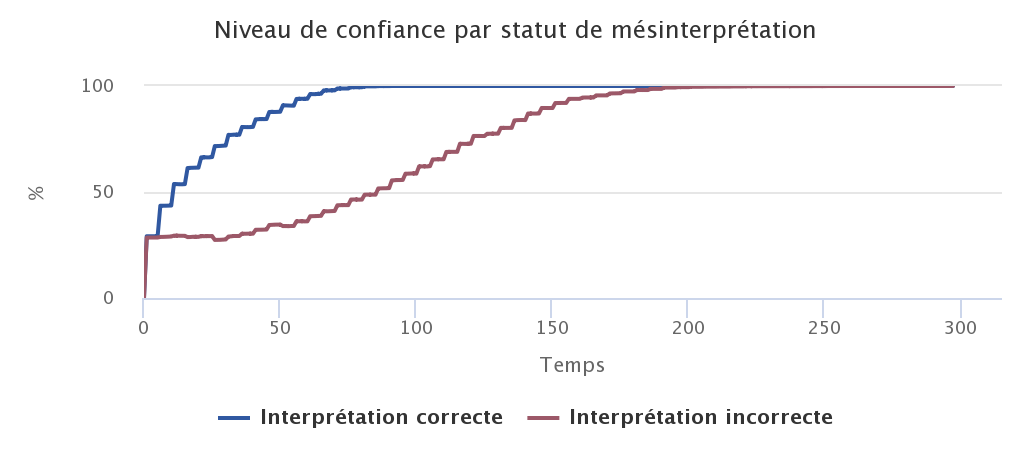
\includegraphics[width=1.0\linewidth]{fig/trust_03_graph_trust_misint.png}
            \end{minipage}
            \\
            \begin{minipage}[t]{0.3\textwidth}
                \vspace{1.5mm}
                Population's initial average trust: \textbf{0.7}
            \end{minipage}
            \begin{minipage}[t]{0.6\textwidth}
                \strut\vspace*{-\baselineskip}\newline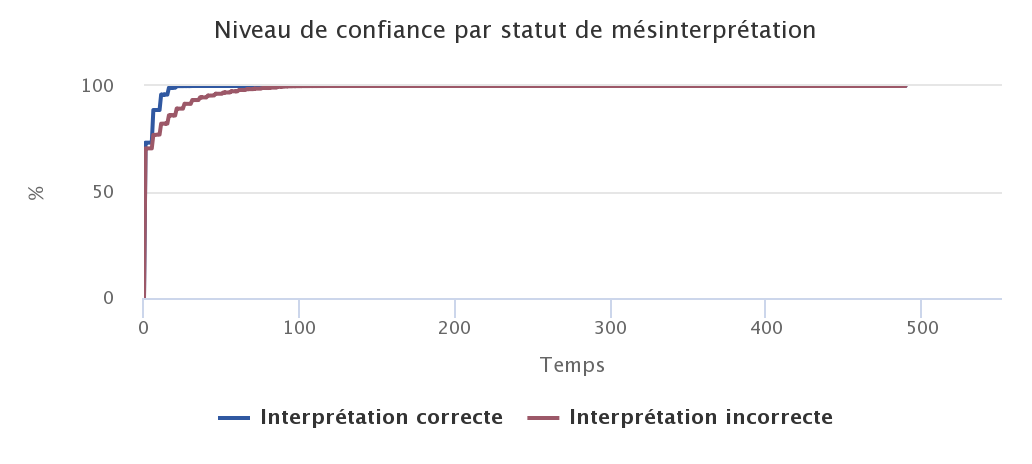
\includegraphics[width=1.0\linewidth]{fig/trust_07_graph_trust_misint.png}
            \end{minipage}
        \end{center}
        \caption{Average trust level per misinterpretation status}
    \end{figure}
\end{frame}

\begin{frame}{Deceased, vaccinated and misinterpretation}
    \begin{figure}[htpb]
        \begin{center}
            \begin{minipage}[t]{0.3\textwidth}
                \vspace{1.5mm}
                Population's initial average trust: \textbf{0.3}
            \end{minipage}
            \begin{minipage}[t]{0.6\textwidth}
                \strut\vspace*{-\baselineskip}\newline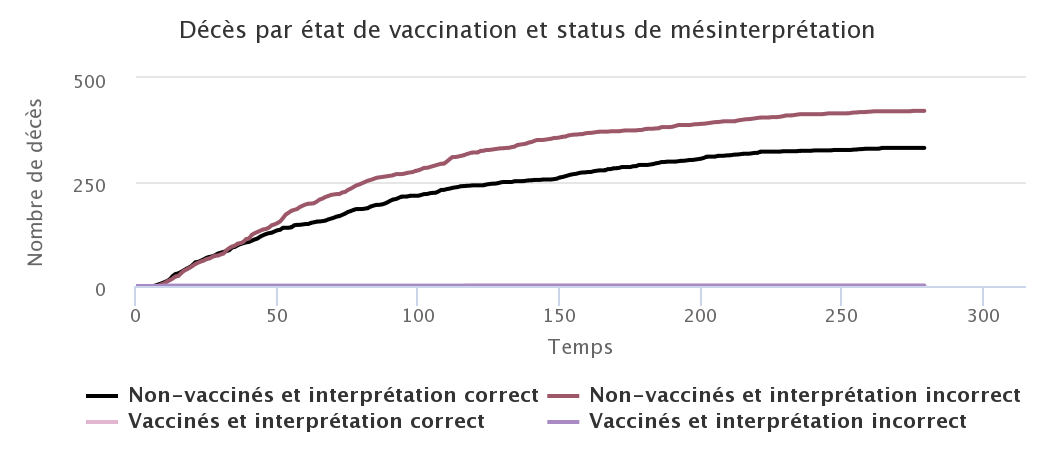
\includegraphics[width=1.0\linewidth]{fig/trust_03_graph_dec_vacc_misint.png}
            \end{minipage}
            \\
            \begin{minipage}[t]{0.3\textwidth}
                \vspace{1.5mm}
                Population's initial average trust: \textbf{0.7}
            \end{minipage}
            \begin{minipage}[t]{0.6\textwidth}
                \strut\vspace*{-\baselineskip}\newline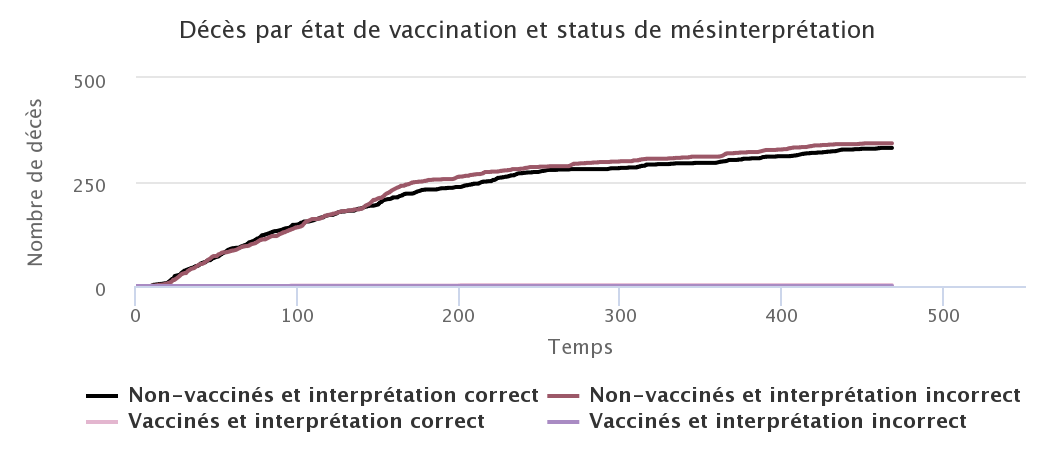
\includegraphics[width=1.0\linewidth]{fig/trust_07_graph_dec_vacc_misint.png}
            \end{minipage}
        \end{center}
        \caption{Deceased per vaccination \& per misinterpretation status}
    \end{figure}
\end{frame}



\section{Discussion}

\begin{frame}{Contribution}
    \begin{itemize}
        \item Combination of epidemiological ABM \& trust in vaccines
        \item Population trust is important and needed before the start of the vaccination campaign
        \item Making sure that the population correctly understands given information is crucial to heighten trust and give people the desire to get vaccinated
    \end{itemize}
\end{frame}

\begin{frame}{Future plans}
    \begin{itemize}
        \item Add age groups
        \item Households (influence trust among families)
        \item Different types of information sources (influence trust differently)
    \end{itemize}
\end{frame}



% \section{References}

% \begin{frame}[allowframebreaks]
%     %\bibliography{ref}
%     \bibliographystyle{alpha}
%     % If there are too many references, you can adjust the font like this:
%     % \tiny\bibliographystyle{alpha}
% \end{frame}

%\begin{frame}{References}
%	\printbibliography[heading=reference]
%\end{frame}



\begin{frame}
    \titlepage
    \begin{figure}[htpb]
        \begin{center}
            \includegraphics[width=0.1\linewidth]{fig/logos/Logo_Université_Grenoble_Alpes_2020.svg.png}\quad\quad
            
\includegraphics[width=0.1\linewidth]{fig/logos/logo_Grenoble_INP.png}\quad\quad
            
\includegraphics[width=0.1\linewidth]{fig/logos/logo_cnrs.png}\quad\quad
            
\includegraphics[width=0.1\linewidth]{fig/logos/Logo_LIG.png}\quad\quad
            
\includegraphics[width=0.1\linewidth]{fig/logos/Logo_GIPSA-lab_Grenoble.jpg}
        \end{center}
    \end{figure}
\end{frame}

\end{document}
